\chapter{Potenza lungo la Linea con Perdite}
Consideriamo il\textbf{ circuito equivalente} associato ad 
una \textbf{fettina dz} di \textbf{linea con perdite}:
\begin{center}
    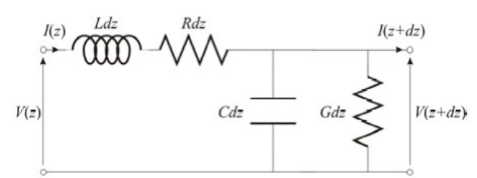
\includegraphics[width=0.8\textwidth]{Images/figure16.png}
\end{center}
Che possiamo sintetizzare nel seguente modo:
\begin{center}
    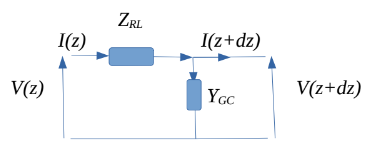
\includegraphics[width=0.8\textwidth]{Images/figure17.png}
\end{center}
Dove:
\begin{itemize}
    \item $Z_{RL} = j\w L_{eq}= j\w \left(L -     j\frac{R}{\w}  \right) = j\w L + R$
    \item $Y_{GC} = j\w C_{eq}= j\w \left(C -     j\frac{G}{\w}  \right) = j\w C + G$
\end{itemize}
\textbf{Risolvendo} il circuito ottengo:
\begin{equation*}
\tag{Tensione}
    V(z + dz) - V(z) = -Z_{RL} dz I = - j \w L_{eq} dz I
\end{equation*}
Quindi:
\begin{equation*}
    \frac{dV}{dz} = - j \w L_{eq} I
\end{equation*}
\begin{equation*}
\tag{Corrente}
    I(z + dz) - I(z) = -Y_{GC} dz V = - j \w C_{eq} dz V
\end{equation*}
Quindi:
\begin{equation*}
    \frac{dI}{dz} = - j \w C_{eq} V
\end{equation*}
\section{Linea Indefinita}
In particolare valutiamo la seguente situazione:
\begin{center}
    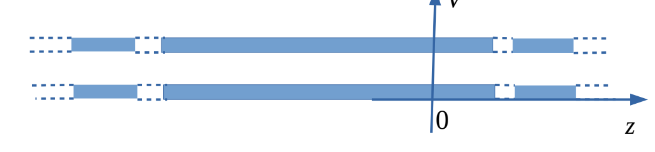
\includegraphics[width=0.8\textwidth]{Images/figure18.png}
\end{center}
Dove avremo il seguente andamento di \textbf{tensione} e \textbf{corrente}:
\begin{equation*}
    \begin{dcases}
    V(z) = V^+ e^{-jkz} + V^- e^{jkz}\\
    I(z) = \frac{V^+}{Z_0} e^{-jkz} + \frac{V^-}{Z_0} e^{jkz}
    \end{dcases}
\end{equation*}
Dove:
\begin{equation*}
\begin{aligned}
    k &= \w \sqrt{L_{eq} C_{eq}} = \w \sqrt{\left(L - j\frac{R}{\w} \right) \left(C - j\frac{G}{\w}  \right)} =  \\
    &=\w \sqrt{\left(LC - \frac{RG}{\w^2} \right)- j\left(\frac{LG}{\w} + \frac{RC}{\w} \right)}
\end{aligned}
\footnote{fai la moltiplicazione e poi separa Re e Im}
\end{equation*}
Quindi:
\begin{equation*}
    k = \beta - j \alpha
\end{equation*}
E consideriamo il solo \textbf{caso fisico}:
\begin{equation*}
    \beta >0 \ , \quad \alpha >0
\end{equation*}
\begin{equation*}
    V(z) = V^+ e^{-jkz} = V^+ e^{-j(\beta - j\alpha )z} = |V^+| e^{j\alpha_+} e^{-\alpha z} e^{-j\beta z} 
\end{equation*}
E passiamo nel \textbf{dominio del tempo}:
\begin{equation*}
    v(z,t) = |V^+| e^{-\alpha z} \cos(\w t + \alpha_+ - \beta z)
\end{equation*}
Che con $\beta>0$ e $\alpha>0$ rappresenta \textbf{un'onda} che si propaga con \textbf{velocità} $v = \frac{\w}{\beta}$ nelle z positive \textbf{attenuandosi}.\\ \\
Complessivamente la \textbf{tensione} sarà:
\begin{equation*}
    V(z) = V^+ e^{-jkz} + V^- e^{jkz} = V^+ e^{-\alpha z} e^{-j\beta z} + V^- e^{-\alpha z} e^{j\beta z}
\end{equation*}
Calcoliamoci $Z_0$:
\begin{equation*}
    Z_0 = \sqrt{\frac{L_{eq}}{C_{eq}}} = \sqrt{\frac{L - j \frac{R}{\w}}{C - j \frac{G}{\w}}} = \sqrt{\frac{L}{C} \ \frac{1 - j \frac{R}{\w L} }{1 - j \frac{G}{\w C}}}
\end{equation*}
$Z_0$ sarà sempre \textbf{reale} e \textbf{positivo} se vale:
\begin{equation*}
\tag{HEAVISIDE}
    \frac{R}{\w L} = \frac{G}{\w C} 
\end{equation*}
In tal caso:
\begin{equation*}
    Z_0 = \sqrt{\frac{L}{C}} 
\end{equation*}
Se L, C, R e G \textbf{non dipendono dalla frequenza} allora:
\begin{itemize}
    \item $\beta = \w \sqrt{LC}$
    \item $\alpha = - \sqrt{\frac{L}{C}} G$
\end{itemize}
Tuttavia la condizione di \textbf{HEAVISIDE} è difficile da verificarsi, quindi nel caso in cui non si verifichi, la scelta \textbf{corretta} è quella di $Re\{Z_0\} >0$:
\begin{equation*}
    \begin{dcases}
    V(z) = V^+ e^{-j(\beta - j\alpha)z}\\
    I(z) = \frac{V^+}{Z_0} e^{-j(\beta - j\alpha)z}
    \end{dcases}
\end{equation*}
Calcolo la \textbf{Potenza}:
\begin{equation*}
    P(z) = \frac{1}{2} V(z) I^*(z) = \frac{1}{2} \frac{|V^+|^2}{Z_0^*} e^{-2\alpha z}
\end{equation*}
Suddivido in \textbf{potenza attiva} e \textbf{potenza reattiva}:
\begin{equation*}
    P(z) = \frac{1}{2} \frac{|V^+|^2}{\left(\frac{|Z_0|^2}{Z_0}\right)} e^{-2\alpha z} = \frac{1}{2} \frac{|V^+|^2}{R_0^2 +X_0^2} (R_0 + j X_0) e^{-2\alpha z}
\end{equation*}
\begin{equation*}
    P_R(z) =  \frac{1}{2} \frac{|V^+|^2}{R_0^2 +X_0^2}R_0 e^{-2\alpha z}
\end{equation*}
Che è una \textbf{potenza positiva} e \textbf{diminuisce} al \textbf{crescere} \textbf{di} \textbf{z}.\\ \\
\section{Potenza tra due ascisse}
Per capire meglio analizziamo il seguente caso:
\begin{center}
    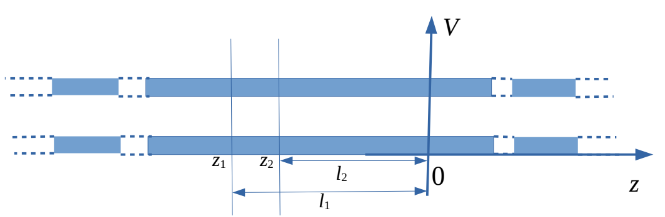
\includegraphics[width=0.8\textwidth]{Images/figure19.png}
\end{center}
Dove avremo le seguenti \textbf{potenze}:
\begin{equation*}
    \begin{dcases}
    P_R(z_1) = \frac{1}{2}\frac{|V^+|^2}{|Z_0|^2} R_0 e^{-2\alpha z_1}\\
    P_R(z_2) = \frac{1}{2}\frac{|V^+|^2}{|Z_0|^2} R_0 e^{-2\alpha z_2}
    \end{dcases}
\end{equation*}
\begin{equation*}
\begin{aligned}
    P_R(z_1) - P_R(z_2) &= \frac{1}{2}\frac{|V^+|^2}{|Z_0|^2} R_0 e^{-2\alpha z_1} - \frac{1}{2}\frac{|V^+|^2}{|Z_0|^2} R_0 e^{-2\alpha z_2} = \\
    &= \frac{1}{2}\frac{|V^+|^2}{|Z_0|^2} R_0\left(e^{2\alpha l_1} - e^{2\alpha l_2}\right)
\end{aligned}
\end{equation*}
La \textbf{differenza delle due potenze attive} rappresenta la \textbf{potenza dissipata dalla linea tra le due sezioni} ed è positiva (quindi $R_0 >0$, $\alpha>0$).\\ \\
Ripetiamo il calcolo per $P_x$:
\begin{equation*}
    \begin{dcases}
    P_X(z_1) = \frac{1}{2}\frac{|V^+|^2}{|Z_0|^2} X_0 e^{-2\alpha z_1}\\
    P_X(z_2) = \frac{1}{2}\frac{|V^+|^2}{|Z_0|^2} X_0 e^{-2\alpha z_2}
    \end{dcases}
\end{equation*}
\begin{equation*}
\begin{aligned}
    P_X(z_1) - P_X(z_2) &= \frac{1}{2}\frac{|V^+|^2}{|Z_0|^2} X_0 e^{-2\alpha z_1} - \frac{1}{2}\frac{|V^+|^2}{|Z_0|^2} X_0 e^{-2\alpha z_2} = \\
    &= \frac{1}{2}\frac{|V^+|^2}{|Z_0|^2} X_0\left(e^{2\alpha l_1} - e^{2\alpha l_2}\right)
\end{aligned}
\end{equation*}
La \textbf{differenza tra le potenze reattive} è \textbf{proporzionale alla differenza delle pseudo energie elettriche e magnetiche medie immagazzinate nel tratto di linea}.\\ \\
Tale \textbf{potenza} è \textbf{positiva} o \textbf{negativa} in base al segno di $X_0$ (discorso analogo per $V^-$).\\ \\
Consideriamo ora:
\begin{equation*}
\begin{aligned}
    k &= \w \sqrt{\left(LC - \frac{RG}{\w^2} \right)- j\left(\frac{LG}{\w} + \frac{RC}{\w} \right)} =\\
    &=\w \sqrt{LC}\sqrt{1 - \frac{RG}{\w^2 LC} - j\left(\frac{G}{\w C} + \frac{R}{\w L} \right) }
\end{aligned}
\end{equation*}
Avere \textbf{piccole perdite} vuol dire:
\begin{itemize}
    \item $\frac{R}{\w L} << 1 \implies \frac{RG}{\w^2 LC} << \frac{R}{\w L}$\\
     \item $\frac{G}{\w C} << 1 \implies \frac{RG}{\w^2 LC} << \frac{G}{\w C}$
\end{itemize}
Queste approssimazioni ci \textbf{semplificano} l'espressione di k:
\begin{equation*}
    k \approx \w \sqrt{LC} \left(1 - j \frac{1}{2} \left(\frac{G}{\w C} + \frac{R}{\w L}\right)\right) = \beta  - j \alpha
\end{equation*}
Quindi $\beta$ ha lo steso valore di \textbf{k} in \textbf{assenza di perdite}, ma esse danno luogo ad un'\textbf{attenuazione} che cresce \textbf{linearmente} con le \textbf{perdite}.\\ \\
Calcoliamo ora l'\textbf{impedenza caratteristica}:
\begin{equation*}
\begin{aligned}
    Z_0 &= \sqrt{\frac{L_{eq}}{C_{eq}}} = \sqrt{\frac{L - j \frac{R}{\w}}{C - j \frac{G}{\w}}} = \sqrt{\frac{L}{C} \frac{1 - j \frac{R}{\w L}}{1 - j \frac{G}{\w C}}} =\\
    &= \sqrt{\frac{L}{C}} {\left(1 - j \frac{R}{\w L}\right)}^{1/2}{\left(1 - j \frac{G}{\w C}\right)}^{-1/2}
\end{aligned}
\end{equation*}
Nel caso di \textbf{piccole perdite}:
\begin{equation*}
    \frac{R}{\w L} << 1 \implies {\left(1 - j \frac{R}{\w L}\right)}^{1/2} \approx 1 - j \frac{1}{2} \frac{R}{\w L}
\end{equation*}
E dato che:
\begin{equation*}
    \frac{G}{\w C} << 1 \implies {\left(1 - j \frac{G}{\w C}\right)}^{1/2} \approx 1 + j \frac{1}{2} \frac{G}{\w C}
\end{equation*}
Quindi sostituendo:\footnote{Trascuro il termine con il coefficiente $\frac{1}{4}$}
\begin{equation*}
    Z_0 = \sqrt{\frac{L}{C}} + j \frac{1}{2} \sqrt{\frac{L}{C}} \left(\frac{G}{\w C} - \frac{R}{\w L} \right) = R_0 + j X_0
\end{equation*} 
Dove:
\begin{itemize}
    \item $R_0 = \sqrt{\frac{L}{C}}$
    \item $X_0 = \frac{1}{2} \sqrt{\frac{L}{C}} \left(\frac{G}{\w C} - \frac{R}{\w L} \right)$
\end{itemize}
Quindi ha la \textbf{parte reale} uguale a come sarebbe $Z_0$ in \textbf{mancanza di perdite}, o nel caso in cui valga la \textbf{condizione di Heaviside}.\\ \\
\section{Linea con Carico}
Infine consideriamo la seguente situazione:
\begin{center}
    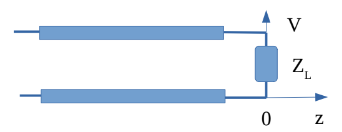
\includegraphics[width=0.5\textwidth]{Images/figure20.png}
\end{center}
Dove:
\begin{equation*}
    \begin{dcases}
    k = \beta - j \alpha\\
    Z_0 = R_0 + j X_0
    \end{dcases}
\end{equation*}
\begin{equation*}
\begin{aligned}
    V(z) &= V^+ e^{-\alpha z} e^{-j\beta z} + V^- e^{\alpha z} e^{j\beta z} = \\
    &= V^+ e^{-\alpha z} e^{-j\beta z} \left(1 + \frac{V^-}{V^+} e^{2\alpha z} e^{2j\beta z}\right) = V^+ e^{-\alpha z} e^{-j\beta z} \left(1 + \Gamma(z)\right)\\
    I(z) &= \frac{V^+}{Z_0} e^{-\alpha z} e^{-j\beta z} \left(1 - \Gamma(z)\right)
\end{aligned}
\end{equation*}
\begin{equation*}
    \Gamma(0) = \Gamma_l = \frac{V^-}{V^+} = \frac{Z_l - Z_0}{Z_l + Z_0}
\end{equation*}
Nel caso di piccole perdite $X_0 << R_0$, quindi:
\begin{equation*}
    \Gamma(0) = \frac{Z_l - R_0 - j X_0}{Z_l + R_0 + j X_0} \approx \frac{Z_l - R_0}{Z_l + R_0} - j \underbrace{\frac{X_0}{R_0} \frac{1}{\frac{Z_l}{R_0} + 1}}_{trascurare}
\end{equation*}
La differenza maggiore dal caso \textbf{senza perdite} è che $|\Gamma(z)| =|\Gamma(0)| e^{2\alpha z} $ \textbf{non è costante} lungo la linea, ma allontanandosi dal \textbf{carico}, il modulo \textbf{diminuisce}.\\ \\
Calcoliamo ora la generica potenza lungo la linea:\footnote{$|\Gamma(z)| = |\Gamma_L| e^{2\alpha z}$}\footnote{$\Gamma(z) = \Gamma_L e^{2\alpha z} e^{2j\beta z}$}
\begin{equation*}
    \begin{aligned}
    P(z) &= \frac{1}{2} V(z) I^*(z) = \frac{1}{2} V^+ e^{-\alpha z} e^{-j \beta z} \left(1 + \Gamma(z) \right) \frac{{V^+}^*}{Z_0^*}e^{-\alpha z} e^{j \beta z} \left(1 - {\Gamma(z)}^* \right) =\\
    &= \frac{1}{2} \frac{|V^+|^2}{Z_0^*} e^{-2\alpha z}\left(1 - |\Gamma(z)|^2 + \Gamma(z) - {\Gamma(z)}^* \right) =\\
    &= \frac{1}{2} \frac{|V^+|^2}{Z_0^*} e^{-2\alpha z}\left(1 - |\Gamma(z)|^2 +2j Im\{\Gamma(z)\} \right) =\\
    &= \frac{1}{2} \frac{|V^+|^2}{Z_0^*} e^{-2\alpha z}\left(1 - |\Gamma_l|^2 e^{4\alpha z}\right) + j  \frac{|V^+|^2}{Z_0^*} e^{-2\alpha z}e^{2\alpha z} Im\{\Gamma_l e^{2j\beta z}\}=\\
    &= \underbrace{\frac{1}{2} \frac{|V^+|^2}{Z_0^*} e^{-2\alpha z}\left(1 - {|\Gamma_l|}^2 e^{4\alpha z}\right)}_{\text{P. onda dir.\ meno P. onda rifl.}} + j  \frac{{|V^+|}^2}{Z_0^*}Im\{\Gamma_l e^{2j\beta z}\}
    \end{aligned}
\end{equation*}

Allontanandosi dal carico la \textbf{potenza} \textbf{dell'onda riflessa} sarà sempre più \textbf{piccola} di quella dell'\textbf{onda incidente}.






